\documentclass[a4paper,11pt]{article}

\usepackage{graphicx}
<<<<<<< HEAD
\usepackage{subfig,hyperref}
\newcommand{\HRule}{\rule{\linewidth}{0.5mm}}

\begin{document}
\pagenumbering{alph}
\begin{titlepage}
\begin{center}

\textsc{\LARGE CMSC726 Machine Learning}\\[1.5cm]

\textsc{\Large Project 2}\\[0.5cm]

\HRule \\[0.5cm]

{ \huge \bfseries Complex Classification}\\[0.4cm]

\HRule \\[1.5cm]

{\large Angjoo Kanazawa, Ran Liu, and Austin Myers}

\vfill

{\large November 1, 2011}

\end{center}
\end{titlepage}
%\title{ML CS726 Fall'11 Project 2 Complex Classifiers}
%\author{Angjoo Kanazawa, Ran Liu, Austin Myers}
%\maketitle
\pagenumbering{arabic}

\section{PCA and Kernel PCA}
\subsection{WU1}
\textsf{Depending exactly on your random data, one or more of these lines might not pass exactly through the data as we would like it to. Why not?}\\


\subsection{WU2}
\textsf{Plot the normalized eigenvalues (include the plot in your writeup). How many eigenvectors do you have to include before you've accounted for 90\% of the variance? 95\%? (Hint: see function cumsum.)}\\

% \begin{figure}[!ht]
%   \begin{center}
%   \caption{Plot of the normalized eigenvalues}
%   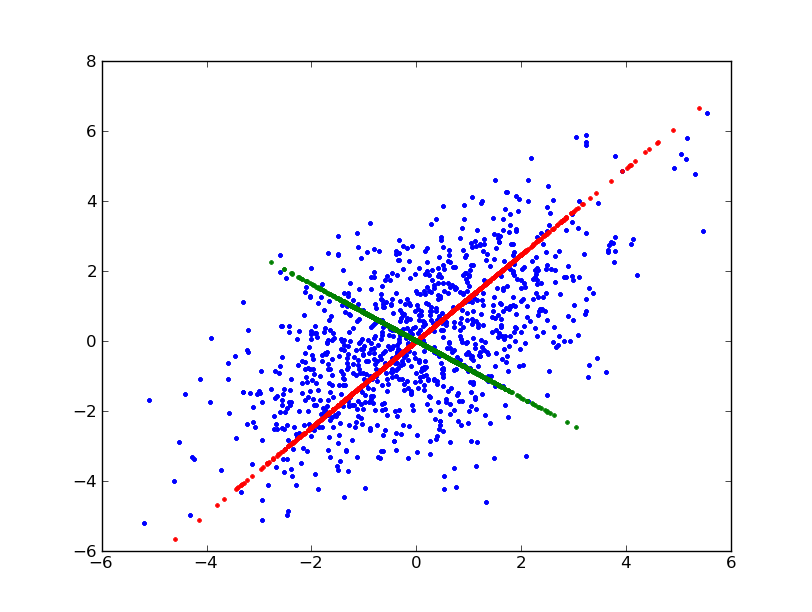
\includegraphics[width=4.5in]{pca.png}
%   \label{figures:wu61}
%   \end{center}
% \end{figure}

\subsection{WU3}
\textsf{Do these look like digits? Should they? Why or why not?
(Include the plot in your write-up.)}
% \begin{figure}[!ht]
%   \begin{center}
%   \caption{Plot of digits using vanilla pca}
%   \includegraphics[width=4.5in]{pca_digits.png}
%   \label{figures:wu61}
%   \end{center}
% \end{figure}
\subsection{WU4}
\textsf{Why does vanilla PCA find this data difficult? What is the
significance of the relatively large value of the eigenvalues here?}
\subsection{WU5}
\textsf{Did PCA do what we might want it to? Why or why not? Include
the plot to justify your answer.}
% \begin{figure}[!ht]
%   \begin{center}
%   \caption{Pca doing what we want..}
%   \includegraphics[width=4.5in]{pca2.png}
%   \label{figures:wu61}
%   \end{center}
% \end{figure}
\subsection{WU6}
\textsf{How do the eigenvalues here compare to the linear case? What
does this tell you? How does the plot look? How might this be useful
for supervised learning?}
% \begin{figure}[!ht]
%   \begin{center}
%   \caption{Using KPCA}
%   \includegraphics[width=4.5in]{pca2.png}
%   \label{figures:wu61}
%   \end{center}
% \end{figure}
\subsection{WU7}
\textsf{Experiment with different kernels, and perhaps interpolations of different kernels. Try to find a kernel that gets as much of the variance on the first two principle components as possible. Report your kernel and a plot of the data projected into 2d under that kernel.}
\pagebreak
\section{HMMs:Viterbi}
\subsection{WU8}
\textsf{find two different observation sequences of length four that
differ only in one place, but differ in more than one place in the
guessed output.}
hmm.viterbi(array([0,1,1,1]), a, b, pi) # 0 0 0 0
hmm.viterbi(array([0,1,2,1]), a, b, pi) # 0 0 1 1

\section{HMMs:Forward-backward}
\subsection{WU9}
\textsf{Why does EM settle in this configuration? What is it saying? What happens when you use three states instead of two? What's the resulting probability of the data? What about four states? What happens and why?}\\

=======
\usepackage{subfig}


\begin{document}
\title{ML CS726 Fall'11 Project 2 Complex Classifiers}
\author{Angjoo Kanazawa, Ran Liu, Austin Myers}
\maketitle


\section{Gradient Descent and Linear Classification}
\subsection{WU1}
\textsf{Find a few values of step size where it converges and a few
  values where it diverges. Where does the threshold seem to be?}\\
It depends on what the number of iteration is, but with 100
iterations, from step 0.1 to 6.5 it finds a solution close to
0. But right after 6.6, it starts to diverge and for any value after
6.7 it diverges. The treshold seems to be around 6.6.

\subsection{WU2}
\textsf{Come up with a non-convex univariate optimization
  problem. Plot the function you're trying to minimize and show two
  runs of gd, one where it gets caught in a local minimum and one
  where it manages to make it to a global minimum. (Use different
  starting points to accomplish this.)}\\
Using $f(x) = sin(\pi x) + x^2/2$, $f'(x) = \pi cos(\pi x) + x$, and
10 iterations, the
global minimum happens at $x\approx -0.45385$.
If we start at 0, we can find the global minimum, but if we start at
1, gd gets caught in a local minimum $1.357$
\begin{verbatim}
>>> gd.gd(f, derF, 0, 10, 0.2)
(-0.45385351939658519, array([ 0.        , -0.72244765, -0.84494752, -0.88472033, -0.88650671,
       -0.88651822, -0.88651823, -0.88651823, -0.88651823, -0.88651823,
       -0.88651823]))
>>> gd.gd(f, derF, 1, 10, 0.2)
(1.3577434052579487, array([  1.22464680e-16,   4.52961014e-02,   2.50055080e-02,
         2.00175811e-02,   1.99477186e-02,   1.99477147e-02,
         1.99477147e-02,   1.99477147e-02,   1.99477147e-02,
         1.99477147e-02,   1.99477147e-02]))
\end{verbatim}

\subsection{WU3}
\textsf{Why does the logistic classifier produce much larger weights
  than the others, even though they all get basically the same
  classification performance?}\\ Don't have to answer this.

\section{Warm Up with ML Tools}
\label{sec:warmup}
\subsection{WU4}
\textsf{What are the five features with largest positive weight and what
are the five features with largest negative weight? Do these seem "right"
based on the task?}\\

\begin{enumerate}
 \item motif -1.21427941322326660156
 \item window -1.15418136119842529297
 \item server -0.94833439588546752930
 \item list -0.89077484607696533203
 \item x -0.86568439006805419922
\end{enumerate}

\begin{enumerate}
 \item graphics 1.09135174751281738281
 \item images 0.72243607044219970703
 \item image 0.72001230716705322266
 \item card 0.71239823102951049805
 \item xx 0.69124054908752441406
\end{enumerate}

\subsection{WU5}
\textsf{ Draw the tree. How do the selected features compare to the
  features from the logistic regression model? Which features seem
  "better" and why? If you use a depth 10 tree, how well do you do on
  test data?}\\
TODO: add the image of the tree later
The selected features include four of the best/worst features from
the logistic regression (``graphics'', ``motif'', ``window'', and ``x'').

Features can be considered ``better'' when the ratio bewteen class 1
and class 0 at the leaf is higher and when the frequency of the number
of instances that got to that leaf is high. In this respect, ``motif''
and ``vga'' are the better features. ``motif'' has high frequency
(total 583 instances fall have no motif) and high ratio (about 80\% of
those without ``motif'' are in class 1).  395 instances fall in
``vga'', and 84\% of those with no ``vga'' are in class 0. If they
have ``vga'', 100\% of them are in class 1 (although this may not be the
best indicator because only 13 data falls into yes ``vga''.) 
In this respect, ``usr'' is one of the worst features in this tree
because the relative frequency is low, adn when there is no ``usr'',
the ratio of class1 to class0 is 6:4.

If I use a depth 10 tree, I get a test error of 20.53\%, (0.463\%
improvement).

\subsection{WU6}
\textsf{}\\

\subsection{WU7}
\textsf{}\\

\section{Reductions for Multiclass Classification}
\subsection{WU8}
\textsf{}\\

\subsection{WU9}
\textsf{}\\

\subsection{Ranking or Collective Classification}
\subsection{WU10a}
\textsf{}\\


\subsection{WU10b}
\textsf{}\\



      
>>>>>>> 209c82cfd4e372a15cf68b51dbf659dea6ddb79f
\end{document}
